\documentclass[pdf]{beamer}
\usepackage[utf8]{inputenc}
\usepackage{cite}
\usepackage{graphicx}
\usepackage{float}
\usepackage{fontawesome}
\usepackage{multicol}
\usepackage{listings}
\usepackage{array}
\usepackage{subcaption}
\usepackage{multirow}
\usepackage{amsmath}
\usepackage{xcolor}
\usepackage{booktabs}

% Beamer theme settings
\usetheme{Madrid}
\usecolortheme{default}

\title{OR Paper Review \\MaGIC:  Multi-modality Guided Image Completion}
\author{Bruno Sánchez Gómez}
\date{\today}

\setbeamertemplate{footline}{%
    \leavevmode%
    \hbox{%
        \begin{beamercolorbox}[wd=0.2\paperwidth,ht=2.5ex,dp=1.125ex,center]{author in head/foot}%
            \hspace*{2mm}Bruno Sánchez Gómez
        \end{beamercolorbox}%
        \begin{beamercolorbox}[wd=0.7\paperwidth,ht=2.5ex,dp=1.125ex,center]{title in head/foot}%
            \insertshorttitle
        \end{beamercolorbox}%
        \begin{beamercolorbox}[wd=0.1\paperwidth,ht=2.5ex,dp=1.125ex,center]{date in head/foot}%
            \hspace*{-2mm}\insertframenumber{} / \inserttotalframenumber
        \end{beamercolorbox}%
    }%
    \vskip0pt%
}

\begin{document}

\begin{frame}
    \titlepage
\end{frame}


\begin{frame}{Table of Contents}
    \tableofcontents
\end{frame}

\section{Introduction}

\begin{frame}{Image Completion}
    \centering
    \begin{minipage}{0.8\textwidth}
        \begin{block}{Definition}
            \centering
            \textit{Image completion} refers to the task of filling in missing regions within an image in a visually plausible way.
        \end{block}
    \end{minipage}
    \vspace{0.5cm}
    \begin{itemize}
        \item \textbf{Applications:}
            \begin{itemize}
                \item \textbf{Inpainting:} Restoring damaged or missing parts of an image.
                \item \textbf{Outpainting:} Extending the boundaries of an image.
                \item \textbf{Editing:} Modifying images by adding or removing elements.
            \end{itemize}
        \item \textbf{Approaches:}
            \begin{itemize}
                \item \textbf{Vanilla Image Completion:} Relies solely on existing image pixels around the masked region.
                \item \textbf{Guided Image Completion:} Uses external cues (e.g., text descriptions, edge maps, segmentation masks) for guidance.
            \end{itemize}
    \end{itemize}
\end{frame}

% \begin{frame}{Approaches to Image Completion}
%     \begin{itemize}
%         \item \textbf{Vanilla Image Completion:}
%         \begin{itemize}
%             \item Relies solely on existing image pixels around the masked region.
%             \item Struggles with large missing areas due to limited internal context.
%             \item Often leads to blurry or repetitive textures.
%         \end{itemize}
%         \item \textbf{Guided Image Completion:}
%         \begin{itemize}
%             \item Uses external cues (e.g., text descriptions, edge maps, segmentation masks) for guidance.
%             \item Improves results significantly, especially for large gaps, by providing external semantic information.
%             \item Existing methods often restricted to \textit{single-modality} guidance, limiting flexibility and performance in complex scenarios requiring multiple constraints.
%         \end{itemize}
%     \end{itemize}
% \end{frame}

\begin{frame}{Multi-modal Guided Image Completion (MaGIC)~\cite{magic}}
    \begin{itemize}
        \item \textbf{MaGIC:} A flexible framework for image completion guided by single or \textit{arbitrary combinations} of modalities, such as:
        \begin{itemize}
            \item Text
            \item Canny Edge
            \item Sketch
            \item Segmentation
            \item Depth
            \item Pose
        \end{itemize}
        \item \textbf{Architecture:} Based on pre-trained stable diffusion (SD) models with a U-Net denoiser.
        \item \textbf{Results:} Outperforms SOTA methods and generalizes well to various completion tasks.
    \end{itemize}
\end{frame}

\section{MaGIC Overview}
\begin{frame}{Table of Contents}
    \tableofcontents[currentsection]
\end{frame}

\begin{frame}{Components of MaGIC}
    \begin{figure}
        \centering
        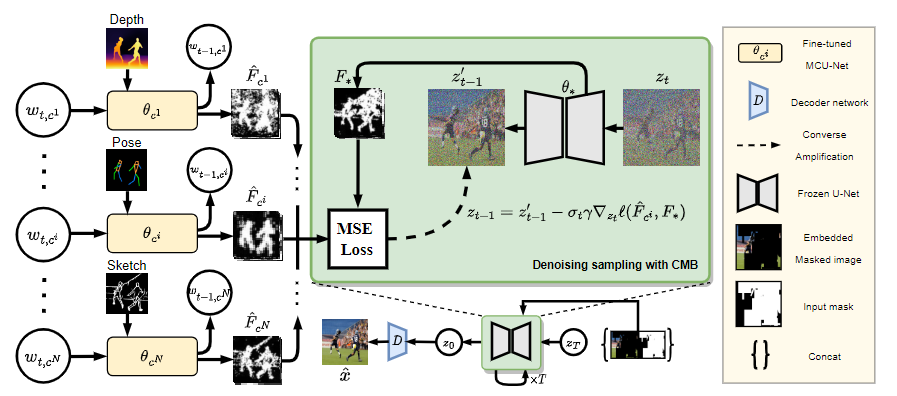
\includegraphics[width=0.75\textwidth]{figures/inference_process.png}
    \end{figure}
    \begin{itemize}
        \item \textbf{Modality-specific Conditional U-Net (MCU-Net):} Injects single-modal guidance into a U-Net denoiser.
        \item \textbf{Consistent Modality Blending (CMB):} Training-free method to blend guidance from multiple pre-trained MCU-Nets, which enables easy addition of new modalities.
    \end{itemize}
\end{frame}

\begin{frame}{Modality-specific Conditional U-Net (MCU-Net)}
    \begin{minipage}{0.65\textwidth}
        \begin{itemize}
            \item The encoding network $\tau_c$ is employed to extract multi-scale guidance signals, $F_c^l$.
            \item Each $F_c^l$ is injected to the latent in MCU-Net to obtain modality-guided features.
            \item To leverage pre-trained SD, the U-Net denoiser is frozen. Only the encoding network $\tau_c$ is trained to extract guidance for the frozen denoiser.
            \item Achieves image completion under single-modality guidance.
        \end{itemize}
    \end{minipage}%
    \begin{minipage}{0.35\textwidth}
        \centering
        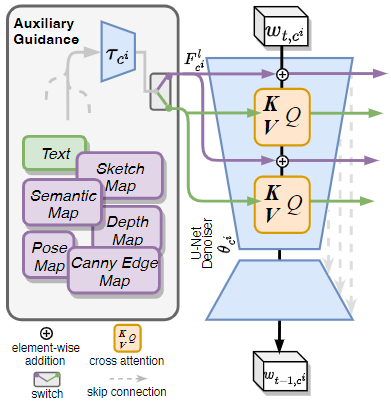
\includegraphics[width=\linewidth]{figures/mcu_net.png}
    \end{minipage}
\end{frame}

\begin{frame}{Consistent Modality Blending (CMB)}
    \begin{itemize}
        \item Uses a \textit{converse amplification strategy}~\cite{dhariwal2021diffusion}, which enables the intermediate feature maps $F_*$ of a original U-Net to more closely approximate the MCU-Nets' guided feature maps $\hat{F}_C$
        \[
        \begin{cases}
            z_{t-1} = z'_{t-1} - \sigma_t \gamma \nabla_{z_t} \ell(\hat{F}_C, F_*)
            \\
            \ell(\hat{F}_C, F_*) = \frac{1}{N \cdot L} \sum\limits_{c\in C} \sum\limits_{l=1}^{L} \delta_c \left\| \hat{F}_c^l - F_*^l \right\|_2^2
        \end{cases}
        \]
        \item \textbf{Properties:}
        \begin{itemize}
            \item It is \textit{training-free}, as it operates on already trained MCU-Nets.
            \item Allows for \textit{arbitraty combination} of available modalities.
            \item Straightforward \textit{integration of new modalities}, by simply training a new MCU-Net for them. Avoids complex joint re-training.
        \end{itemize}
        
    \end{itemize}
\end{frame}

\begin{frame}[shrink=13]{Quantitative Results}
    % FID is a measure of the distance between the distribution of generated images and real images. Lower values indicate better performance.
    % PickScore is a measure of the quality of generated images based on human judgment. Higher values indicate better performance.
    % U-IDS (Unconditional Inception Distance Score) and P-IDS (Perceptual Inception Distance Score) are measures of the diversity of generated images. Higher values indicate better performance.
    \scriptsize
    \vspace{1.2cm}
    \begin{table}[h]
        \centering
        \begin{tabular}{@{}lcccccc@{}}
        \toprule
        \multirow{2}{*}{Method} & \multicolumn{2}{c}{COCO} & \multicolumn{3}{c}{Places2} \\
        \cmidrule(lr){2-3} \cmidrule(lr){4-6}
         & FID$\downarrow$ & PickScore$\uparrow$ / \% & FID$\downarrow$ & U-IDS$\uparrow$ / \% & P-IDS$\uparrow$ / \% \\
        \midrule
        EC (Nazeri et al., 2019) \textcolor{blue}{$\spadesuit$} & 76.64 & 23.14 & 25.08 & 12.89 & 2.86 \\
        CTSDG (Guo et al., 2021) \textcolor{blue}{$\spadesuit$} & 97.05 & 24.03 & 42.81 & 0 & 0 \\
        ZITS (Dong et al., 2022) \textcolor{blue}{$\spadesuit$} & 61.27 & 28.09 & 18.96 & 18.75 & 7.20 \\
        \midrule
        Our MCU-Net$\dagger$ & 47.70$\pm$0.29 & 30.79$\pm$0.10 & 10.74$\pm$0.07 & 23.83$\pm$0.30 & 10.18$\pm$0.48 \\
        Our MCU-Net \textcolor{orange}{$\heartsuit$} & \textbf{39.43$\pm$0.26} & \textbf{37.12$\pm$0.11} & 9.09$\pm$0.04 & 25.34$\pm$0.29 & 10.64$\pm$0.46 \\
        Our MCU-Net \textcolor{red}{$\clubsuit$} & 41.91$\pm$0.20 & 34.96$\pm$0.17 & 10.27$\pm$0.06 & 24.21$\pm$0.24 & 9.93$\pm$0.38 \\
        Our MCU-Net \textcolor{blue}{$\spadesuit$} & 41.15$\pm$0.27 & 34.94$\pm$0.06 & \textbf{8.32$\pm$0.02} & \textbf{26.23$\pm$0.07} & \textbf{10.96$\pm$0.33} \\
        \bottomrule
        \end{tabular}
        \caption{Comparison of using single auxiliary modality as guidance for image completion. \textcolor{blue}{$\spadesuit$}: ground truth edge map as guidance, \textcolor{orange}{$\heartsuit$}: estimated depth map as guidance, \textcolor{red}{$\clubsuit$}: segmentation map as guidance, $\uparrow$: the higher the better, $\downarrow$: the lower the better, $\dagger$: completion without any guidance.}
    \end{table}
\end{frame}

\begin{frame}{Qualitative Results}
    Image examples from the paper
\end{frame}

\section{Critical Analysis}
\begin{frame}{Table of Contents}
    \tableofcontents[currentsection]
\end{frame}
\begin{frame}{Why did MaGIC succeed?}
    
\end{frame}

\begin{frame}{Where did MaGIC fail?}

\end{frame}

\begin{frame}{Future Implications [Placeholder]}
    \begin{itemize}
        \item \textbf{Generalization:} MaGIC's framework can be applied to other image generation tasks, such as inpainting or super-resolution.
        \item \textbf{Modality Fusion:} The CMB method can be extended to fuse more complex modalities, such as audio or video.
        \item \textbf{Real-world Applications:} Potential applications in fields like medical imaging, autonomous driving, and augmented reality.
    \end{itemize}
\end{frame}

\begin{frame}{Q\&A}
    \centering
    \Huge{Thank you for your attention!}

    \vspace{0.5cm}

    \Large{Any questions?}
\end{frame}
\begin{frame}[allowframebreaks]{References}
    \bibliographystyle{unsrt} % Or choose another style like unsrt, alpha, etc.
    \bibliography{references}
\end{frame}

\end{document}